\documentclass[11pt]{article}
\usepackage[margin=1in]{geometry}
\usepackage{amsmath,amssymb,booktabs,longtable,hyperref}
\usepackage{tikz}
\usepackage{graphicx}
\usepackage{microtype}
\usetikzlibrary{arrows.meta,positioning}
\title{Bounded Autonomy Through Environmental Composition:\\An Experimental Study of the GRAIL Runtime}
\author{Mike Amundsen\\Independent Researcher\\\texttt{mca@mamund.com}\\\href{https://orcid.org/0000-0002-9681-8338}{ORCID: 0000-0002-9681-8338}}
\date{Publication candidate v1.4 --- 27 October 2026}
\hypersetup{
  pdftitle={Bounded Autonomy Through Environmental Composition: An Experimental Study of the GRAIL Runtime},
  pdfauthor={Mike Amundsen},
  pdfsubject={Bounded autonomy, environmental composition, experimental evaluation of GRAIL},
  pdfkeywords={GRAIL, bounded autonomy, environmental composition, affordances, reproducibility}
}
\begin{document}
\maketitle
\begin{abstract}
This study investigates whether explicitly composed, bounded environments can support goal-directed autonomous behavior without a general-purpose planning agent. The GRAIL runtime chooses unresolved conditions and affordances, invokes externally implemented capabilities, and updates an internal responsibility-oriented worldstate from reported outcomes. The analysis examines runtime source and a 37-suite regression record alongside eleven recorded scenario executions spanning six experiments: fallback, nested pursuits, three purchasing decisions, a dependency cycle with control, a false-success trust-boundary test with control, and an action-scoped failure-memory test with control. The positive cases demonstrate goal pursuit, alternative selection, recursive delegation, and heterogeneous bindings. Boundary cases show a cyclic pursuit failing to terminate within a three-second observation window, internal goal attainment without a corresponding external effect, and affordance-wide exclusion after a recorded failure. The paper proposes a preliminary operational semantics that distinguishes internal state from external domain truth and limits claims about termination, correctness, and generality. These observations support a bounded account of autonomy through environmental composition, not a universal correctness or performance guarantee.
\end{abstract}
\section{Introduction}
A system may act toward a goal without generating a global plan. In GRAIL, the environment defines conditions to satisfy, affordances that may produce them, and the capabilities that implement those affordances. The research question is: To what extent can autonomous behavior arise from environmental constraints and local decision-making without requiring a general-purpose planning or reasoning agent?

The study examines the narrower empirical proposition that a bounded, explicitly composed environment can support demonstrable goal pursuit, alternative selection after failure, and recursive delegation. These examples do not establish universal autonomy.

\subsection{Research contributions and scope}
This paper makes three contributions. First, it articulates \emph{bounded operational autonomy through environmental composition} as a specific division of responsibilities: a world declares possibilities, prerequisites, and effects; a scenario supplies intent; and a coordinator chooses an unmet need and a means of addressing it, while capabilities implement domain operations. The claim concerns delegated decision authority within a finite authored choice set, not general intelligence or a novel invention of precondition/effect representations.

Second, six experiments provide executable feasibility evidence. E1 demonstrates local alternative selection after failure; E2 demonstrates one form of recursive world composition and distinguishes successful responsibility completion from favorable domain outcomes; E3 demonstrates the same purchasing goal under approval, rejection, and deferral using heterogeneous bindings. These cases show that an LLM is not required in the coordination mechanism, although particular capabilities may use an LLM or human judgment.

Third, three experiments characterize boundaries of the architecture. E4 records a cyclic dependency that exceeds an external timeout, limiting any general termination claim. E5 shows internal goal attainment without a corresponding external effect when a capability falsely reports success. E6 shows affordance-wide failure exclusion across declared effects in the tested pursuit. These negative and controlled cases qualify the positive demonstrations rather than serving as implementation defects to conceal.

The study does \emph{not} claim that the constituent mechanisms are new, that GRAIL outperforms workflow engines or planners, or that its monetary or engineering costs are lower. Architectural economy is a plausible motivation: coordination can avoid mandatory language-model inference, but environment authoring and capability development remain costs to be measured. The contribution is therefore an \emph{empirically qualified architectural account}, not a comparative performance or cost-effectiveness result.


\section{Theoretical Foundations}
\subsection{Bounded rationality and the authored choice set}
Simon's account of bounded rationality motivates a distinction between unconstrained optimization and decision-making within limited information and alternatives \cite{Simon1955}. GRAIL makes the bounds explicit: its runtime selects from authored conditions and affordances, not from arbitrary actions. This is an architectural analogy, not an assertion that the current randomized selectors implement Simon's satisficing procedure. The world author has already encoded much of the knowledge needed for goal pursuit; local runtime selection does not eliminate this prior design work.
\subsection{Affordances as declared software possibilities}
Gibson's ecological notion of affordances concerns possibilities for action in an environment \cite{Gibson1979}. GRAIL uses the term for declared, machine-readable action possibilities with prerequisites, effects and capability bindings. Unlike ecological affordances, these software affordances are not inferred from physical perception; they are explicitly authored. Norman's treatment of design and action possibilities provides a complementary perspective on making possibilities legible to an actor \cite{Norman1988}. The analogy is useful but must not obscure the difference between real environmental properties and a registry's claims.
\subsection{Situated action, reactive selection, and planning}
Brooks' critique of centralized representations and Suchman's analysis of situated action motivate the question of how behavior emerges through local interaction rather than only from precomputed global plans \cite{Brooks1991,Suchman1987}. GRAIL remains a symbolic, goal-oriented runtime, however, and is not equivalent to Brooks' subsumption architecture. Its explicit prerequisites and effects also recall classical action models such as STRIPS \cite{FikesNilsson1971}. The paper's proposed contribution is not the invention of precondition/effect modeling, but an empirical account of bounded coordination using two local selectors, external capability bindings, observations and a deliberate trust boundary.
\subsection{Working definition}
Here, \emph{bounded autonomy} denotes the runtime's ability to choose intermediate needs and available means, react to invocation feedback, and continue or stop a pursuit within an explicitly composed environment, without a human specifying each invocation sequence. This definition does not entail global optimality, independent verification of external effects, or invention of new capabilities.
\section{Environmental Composition as Bounded Operational Autonomy}
\subsection{From prescribed paths to authored possibility spaces}
Environmental composition shifts part of the engineering task from specifying a sequence of operations to specifying the circumstances under which operations can become relevant. A GRAIL \emph{world} declares conditions, affordances, prerequisites, effects, and bindings to operational capabilities. A \emph{scenario} supplies a goal, initial worldstate, and inputs; \emph{observations} preserve a record of attempted and completed activity. These three artifacts separate what may happen, what is sought, and what was reported to have happened. The distinction does not eliminate programming: authors must still design the world and implement capabilities. It instead changes what is fixed before execution. A workflow may prescribe a path, whereas a composed world may admit several paths that become distinguishable only during a pursuit. This is a contrast with path-prescriptive workflows, not with every workflow technology: declarative workflow systems and planning formalisms also allow runtime choice.

The value of composition therefore cannot rest on the novelty of preconditions and effects alone. STRIPS already represented actions through conditions and consequences \cite{FikesNilsson1971}. GRAIL provides a concrete coordination architecture in which those declarations are paired with executable, independently implemented capabilities, two localized selection decisions, and inspectable pursuit observations. The claim examined here is modest: that this arrangement is sufficient to produce useful goal-directed behavior in several bounded software environments without requiring a general-purpose planner in the coordination runtime.

\subsection{Possibility, eligibility, and reported consequence}
Three elements define the immediate decision space. \emph{Possibility} concerns the affordances the author makes available: the runtime cannot select an action that the world does not declare. \emph{Eligibility} concerns prerequisites and available inputs: a declared action may exist but not yet be invocable. \emph{Consequence} concerns effects credited to a successful invocation: these change GRAIL's internal account of which responsibilities have been fulfilled. These are separable obligations. An affordance may be available in the registry but blocked by an unmet prerequisite; a capability may return an unfavorable business decision while successfully fulfilling its declared responsibility; and a capability may report success without producing a corresponding external change.

This last case is not a minor implementation detail. The internal state records what the runtime has reason to credit based on declared effects and reported invocation results. It does not constitute an independently verified description of the external domain. Experiment E5 makes this distinction observable: both scenarios reach the internal goal \texttt{recordCreated}, but only the truthful-success control produces an external record. Thus the environment's composition establishes a boundary for action and attribution, not a universal guarantee about external truth.

\subsection{Two local decisions: needs and means}
GRAIL separates selection of an unmet condition---a \emph{need}---from selection of an affordance capable of satisfying it---a \emph{means}. This separation matters because a pursuit need not commit in advance to one complete invocation sequence. Different unmet conditions may be selected, and a selected condition may have multiple candidate producers. The runtime can also use feedback from a failed invocation to exclude a previously attempted affordance and choose an alternative. E1 records two such fallback events during one successful pursuit; E6 shows that failure exclusion can apply to a multi-effect affordance even when a different declared effect is subsequently needed.

This constitutes \emph{bounded operational autonomy}: authority to choose intermediate needs and means, and to respond to execution feedback, within an authored environment. Autonomy here refers to consequential delegated choice, not to the intelligence, optimality, or novelty of the selection policy. The inspected implementation uses randomized choice among eligible candidates with failure-based filtering; it does not implement a general-purpose planning algorithm or demonstrate adaptive learning. A choice can be operationally meaningful even when the selection rule is simple. Conversely, meaningful choice does not imply that the rule is efficient or that it will terminate on every world. E4's cyclic prerequisites caused repeated resolution attempts until an external timeout, illustrating a structural boundary of this autonomy.

\subsection{Intellectual precedents and the location of complexity}
This account draws on, rather than displaces, earlier work. Simon's bounded rationality locates decisions within limits on available alternatives and information \cite{Simon1955}; his analysis of complex systems motivates attention to modular organization \cite{Simon1962}. The relevance to GRAIL is architectural: much of the coordination problem is constrained before runtime by the environment author. This does not show that the selectors themselves implement Simon's theory of satisficing. Gibson's notion of affordances identifies action possibilities relative to an environment \cite{Gibson1979}, while Norman emphasizes the design and legibility of possible actions \cite{Norman1988}. GRAIL's affordances are explicit software declarations, not ecological affordances perceived directly in a physical world.

Maes' work on situated agents with goals offers a closer precedent for goal-directed action selection through local arbitration rather than complete advance planning \cite{Maes1990}. Its activation-based mechanism differs from GRAIL's current selectors, so the comparison supports a family resemblance rather than algorithmic equivalence. Brooks argues against assuming that useful autonomous behavior always requires a comprehensive centralized representation \cite{Brooks1991}; GRAIL nevertheless maintains an explicit symbolic worldstate and action model, and therefore should not be described as representation-free. These connections suggest a shared design question: how much behavior can be obtained by structuring the agent--environment relationship rather than expanding a centralized reasoning mechanism?

The environment also relocates complexity rather than eliminating it. The author must select appropriate responsibilities, encode dependencies, provide alternatives, define bindings, and decide which claims can be trusted. Capabilities retain the work of interpreting domain outcomes, including policies, credentials, human decisions, and external protocols. E2 demonstrates that a parent pursuit can delegate verification to a child world while treating a \texttt{REJECTED} verification result as a completed responsibility. E3 shows a single purchasing world coordinating HTTP, Node, and interactive STDIO across \texttt{approved}, \texttt{rejected}, and \texttt{deferred} decisions without making those domain decisions inside the runtime.

\subsection{Architectural economy as a research motivation}
An important practical motivation is \emph{architectural economy}: using only as much centralized reasoning machinery as routine coordination requires. In the studied worlds, GRAIL's coordination mechanism does not require an LLM. This is a meaningful feasibility result, because it separates goal-directed execution from a dependency on language-model inference. It is not evidence that LLMs are unnecessary in every capability; a capability may use a language model, conventional domain logic, or human judgment while remaining behind the same operational boundary.

Nor do the present experiments establish cost-effectiveness in a comparative economic sense. They contain no controlled measurements of engineering effort, inference expenditure, operating cost, or maintenance burden against alternative architectures. A lightweight coordinator may reduce \emph{runtime coordination cost} while increasing \emph{environment composition cost}: authoring and validating affordances, capabilities, and dependencies can be substantial work. The defensible proposition is therefore that environmental composition \emph{offers a potentially economical route} to bounded agentic solutions, not that it has been shown cheaper or more scalable than workflow engines, planners, or LLM-based agents.

The experiments support a narrower but consequential conclusion. E1--E3 demonstrate autonomous selection, delegated execution, recursive composition, and separation of business outcome from responsibility completion in authored worlds. E4--E6 identify limitations in termination, external verification, and failure-memory scope. Taken together, they indicate that bounded operational autonomy can be achieved through local need-and-means selection over composed possibilities, while the quality and guarantees of that autonomy remain constrained by the environment and the capability trust boundary.
\section{Related Work and Comparative Architecture}
\subsection{Classical planning and action representations}
Classical planning represents actions through preconditions and effects; STRIPS and PDDL are established precedents for this form of declarative modeling \cite{FikesNilsson1971,McDermott1998}. GRAIL does not introduce precondition/effect representations. The operational distinction concerns when a path is determined: planning systems generally search for a plan against an action model, while GRAIL resolves unmet conditions and selects affordances during pursuit. This local approach does not confer global planning guarantees. E4, in which a cyclic dependency repeatedly triggered resolution until an external timeout, is a concrete limitation. The more precise characterization is runtime goal-directed dependency resolution, not general-purpose planning.
\subsection{Workflow and process orchestration}
Workflow systems already support alternatives, synchronization, and sophisticated control-flow structures; workflow-pattern research demonstrates that they cannot be reduced to rigid linear scripts \cite{Aalst2003}. A useful distinction is the authoring abstraction. A process model typically specifies control-flow relationships among activities, whereas a GRAIL environment declares a bounded space of affordances, eligibility conditions, and effects. The runtime chooses needs and means within that space. E1 shows fallback without a prescribed sequence of individual alternatives. This is not evidence of greater expressiveness or lower authoring cost; it is a different allocation of responsibility between environment author and execution mechanism.
\subsection{Situated action and reactive behavior}
Maes's work on situated agents examines goal-directed behavior through action arbitration \cite{Maes1990}; Brooks argues against treating centralized comprehensive representation as a prerequisite for useful behavior \cite{Brooks1991}. These precedents support the plausibility of meaningful local decision-making. GRAIL, however, uses explicit symbolic conditions and effects and does not implement Maes's activation-network mechanism. Behavior trees provide another modular reactive architecture, with explicit tree-structured control and fallback semantics \cite{Colledanchise2018}. GRAIL instead derives local choices from condition/affordance relationships. Both can coordinate modular capabilities; their relative merits require separate comparative study.
\subsection{Agent architectures and delegated reasoning}
Belief--desire--intention architectures distinguish world representations, desired states, and intended courses of action \cite{RaoGeorgeff1995}. GRAIL also represents a worldstate and goal, but its current selectors do not implement a general BDI deliberation cycle. Bounded operational autonomy here means delegated authority to select an unmet need and an eligible means, not authority to invent arbitrary actions or change the environment. Capabilities may use rules, human judgment, or LLMs; the coordinator itself requires no LLM. E3 demonstrates human review within this separation.
\subsection{Architectural economy and limits}
The proposed economy is an allocation of complexity, not its disappearance. Environmental authors supply accurate affordances and constraints; capabilities supply domain semantics and operational effects; the coordinator remains comparatively small. This is compatible with Simon's account of modular complexity \cite{Simon1962}. Yet composition incurs engineering and validation costs. E5 demonstrates that internal goal attainment does not independently verify external effects, and E6 demonstrates conservative action-wide failure exclusion. The evidence therefore establishes feasibility of this composition pattern, not lower monetary cost, greater scalability, or superiority over planners and workflow engines. A cost-effectiveness claim would require matched-task comparisons of engineering effort, runtime overhead, inference expenditure, and maintenance.
\subsection{Positioning}
GRAIL occupies a design space between explicit process orchestration and general-purpose planning or agent deliberation. Its contribution in this study is an empirically qualified account of a particular composition: declared possibilities, condition-based eligibility, two local selectors, delegated capability execution, and reported effects. The positive experiments show feasibility of this coordination pattern; the boundary experiments delimit its guarantees. This combination of formulation, executable evidence, and boundary characterization constitutes the specific contribution claimed here.

\section{Experimental Apparatus}
\subsection{Runtime, world, and scenario}
GRAIL serves as the experimental coordination apparatus rather than as a domain-specific application. A \emph{world} specifies available affordances and their capability bindings; a \emph{scenario} supplies a goal, initial worldstate, and inputs; and \emph{observations} record the resulting experience of a pursuit. This separation permits the same authored possibilities to be exercised under different initial conditions or domain inputs. In the examined examples, the registry expresses dependencies and declared effects rather than a complete ordered workflow. The environment author nevertheless determines the limits of possible action by deciding which affordances exist and what their declarations mean.

A pursuit begins with a named goal and an internal Boolean worldstate representing credited responsibilities. The coordinator attempts to establish unmet conditions using the authored affordances. Each affordance associates a name with prerequisite conditions, one or more declared effects, and a binding to an operational capability. Capabilities implement domain behavior outside the coordination mechanism. The apparatus thus distinguishes the \emph{declaration} that a responsibility can be fulfilled from the \emph{implementation} that attempts to fulfill it. The registry is not an executable proof of its own declarations.


\begin{figure}[ht]
\centering
\resizebox{\linewidth}{!}{%
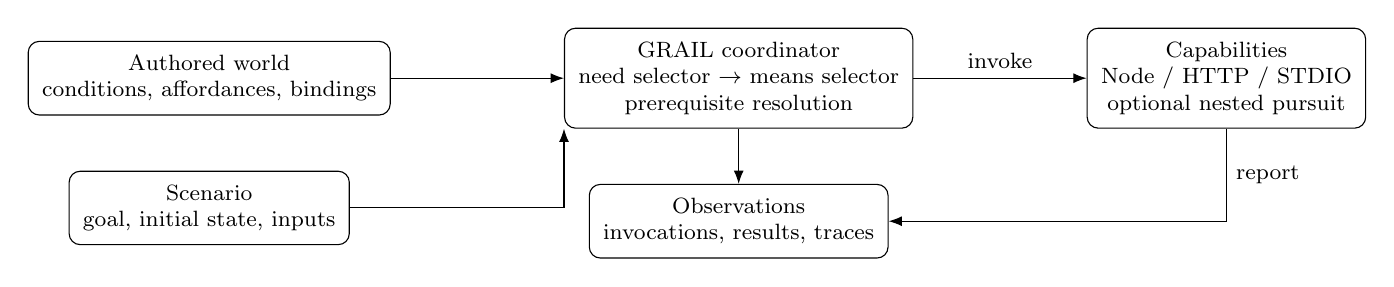
\begin{tikzpicture}[>=Latex, node distance=7mm and 10mm, every node/.style={font=\footnotesize}, box/.style={draw,rounded corners,align=center,minimum height=8mm,inner sep=5pt}]
\node[box] (author) {Authored world\\conditions, affordances, bindings};
\node[box,below=of author] (scenario) {Scenario\\goal, initial state, inputs};
\node[box,right=22mm of author] (runtime) {GRAIL coordinator\\need selector $\rightarrow$ means selector\\prerequisite resolution};
\node[box,below=of runtime] (obs) {Observations\\invocations, results, traces};
\node[box,right=22mm of runtime] (caps) {Capabilities\\Node / HTTP / STDIO\\optional nested pursuit};
\draw[->] (author) -- (runtime);
\draw[->] (scenario.east) -| (runtime.south west);
\draw[->] (runtime) -- node[above]{invoke} (caps);
\draw[->] (caps.south) |- node[near start,right]{report} (obs.east);
\draw[->] (runtime) -- (obs);
\end{tikzpicture}%
}
\caption{Responsibility boundaries in the experimental apparatus. Capability reports update internal credited worldstate; arrows do not imply independent verification of external effects.}
\label{fig:architecture}
\end{figure}

\subsection{Selection and execution}
The inspected runtime exposes two distinct selection points. A need selector chooses an unmet condition to pursue; a means selector chooses an affordance that declares an effect capable of satisfying that condition. In the inspected implementation, both use randomized selection among applicable candidates, with exclusion of some previously failed affordances based on recorded observations. These policies are sufficient to produce different execution paths without a preauthored sequence, but the present study does not claim that they optimize path length, cost, or reliability. The runtime resolves prerequisites before invoking an affordance, records the invocation result, and credits declared effects after reported success. When an invocation fails, an alternative authored affordance may remain available. The execution trace exposes selected conditions, selected affordances, and stack operations; invocation observations capture operational results. Neither record should be mistaken for an independent audit of external state.

\subsection{Capability boundary and composition}
The studied worlds exercise Node module, HTTP, and STDIO bindings, including interactive STDIO for a human purchasing decision. The nested-onboarding world additionally uses an API helper to invoke a child GRAIL pursuit from a parent capability. This is composition through the capability boundary: the parent coordinates a responsibility while the child independently pursues its own goal. The parent receives the child's reported result without needing to implement the child's verification procedure. The same division allows capabilities to return business outcomes such as \texttt{REJECTED}, \texttt{DENIED}, or \texttt{DEFERRED} while reporting successful completion of the responsibility assigned to them. It also creates a trust boundary: internal worldstate reflects reported completion, not necessarily independently verified external consequences.

\subsection{Instrumentation and experimental controls}
The archived evidence consists of scenario configuration files, capability source, complete JSON pursuit outputs, invocation observations, and decision/stack traces. Where relevant, the archives also include persisted domain records and process-harness reports. The boundary experiments add explicit controls. E4 changes an initial prerequisite from satisfied to unsatisfied and imposes an external process timeout; E5 changes whether a record is actually written while retaining a successful capability report; E6 controls selector choices to expose failure exclusion across multiple declared effects. These controls isolate particular architectural behaviors rather than provide statistical samples. The experimental method below specifies the resulting cases and consistency checks.

\subsection{Runtime provenance}
The experiments were assembled from portable world packages and runtime materials that do not all identify the same executable version. E1 and E3 declare \texttt{@mamund/grail} 0.2.0; E2 declares a local \texttt{file:} dependency; separately inspected runtime source and regression results identify 0.3.0-beta.1. Consequently, the apparatus is characterized at the level supported by each archived execution, and the study does not assume binary equivalence across all eleven runs. The version distinction is a reproducibility limitation, not a reason to merge or discard the observations.
\section{Operational Model}
\subsection{Worlds, pursuits, and the trust boundary}
A composed world is modeled as $W=(C,A,\mathrm{pre},\mathrm{eff},\mathrm{bind})$, where $C$ is a finite set of named Boolean responsibility conditions, $A$ is a finite set of authored affordances, $\mathrm{pre}(a)\subseteq C$ gives the prerequisites of action $a$, $\mathrm{eff}(a)\subseteq C$ gives its declared effects, and $\mathrm{bind}(a)$ identifies its operational capability. A scenario supplies $g\in C$, an initial internal worldstate $s_0:C\rightarrow\{0,1\}$, and inputs $i_0$. A condition describes whether GRAIL has credited a responsibility as completed; it need not describe a favorable business outcome.

A pursuit is represented schematically by
\begin{equation}
q=\langle g,s,\kappa,I,O,T,F,m\rangle,
\label{eq:pursuit}
\end{equation}
where $\kappa$ is the obligation stack, $I$ the current input/output environment, $O$ the invocation observations, $T$ the decision/stack trace, $F$ the set of affordance actions excluded by applicable failure observations, and $m$ a control mode. This is an \emph{analytical abstraction}, not a claim that the implementation stores one object with precisely these fields. In particular, $F$ summarizes information drawn from observations rather than requiring a dedicated runtime set.

To expose the trust boundary, let $d\in D$ denote external domain state, which the coordinator does not generally inspect. For a condition $c$, $\mathrm{Ext}(c,d)$ denotes the external proposition an application might intend $c$ to represent. No invariant $s(c)=1\Rightarrow\mathrm{Ext}(c,d)$ is assumed. The model therefore separates \emph{internal responsibility credit} from \emph{external domain truth}.

\subsection{Two decision functions}
Define the producer set of a condition by
\begin{equation}
\mathrm{Prod}(c)=\{a\in A\mid c\in\mathrm{eff}(a)\}.
\end{equation}
For an action $a$ being resolved, its unmet prerequisites are
\begin{equation}
U(a,s)=\{c\in\mathrm{pre}(a)\mid s(c)=0\}.
\end{equation}
The \emph{need selector} chooses $\sigma_N(q,a)\in U(a,s)$ when that set is nonempty. The \emph{means selector} chooses $\sigma_M(q,c)\in\mathrm{Prod}(c)\setminus F$, subject to the runtime's other eligibility and resolution checks. For the initial goal, $c=g$ acts as the unresolved need. The inspected implementation uses randomized choice among available candidates, not a globally optimizing or learned policy. Thus selection is consequential but not evidence of sophisticated deliberation.

A crucial distinction concerns \emph{selection} versus \emph{invocation}. A producer may be selected to address a need even though its prerequisites remain false. The resolver then seeks producers for those prerequisites; it invokes the chosen capability only once the declared prerequisites and required inputs have been resolved. This distinction allows local choices to assemble an execution path incrementally, but it also creates the possibility of unresolved cycles.

\subsection{Abstract transition obligations}
The notation $q\longrightarrow q'$ denotes a coordination step and $\mathrm{report}(a)\in\{\mathrm{SUCCESS},\mathrm{FAIL}\}$ for the outcome reported through a capability binding. The rules below specify the \emph{observable obligations} of the coordination mechanism; they intentionally abstract away individual JavaScript stack operations, input-resolution details, and optional compensation.

\paragraph{Goal recognition (G).} If $s(g)=1$, the pursuit can terminate with $\mathrm{reached}=\mathrm{true}$. This conclusion concerns $s$, not $d$.

\paragraph{Need selection (N).} For a selected action $a$ with $U(a,s)\ne\varnothing$, choose $c=\sigma_N(q,a)$. Record the selection and introduce an obligation to establish $c$ before invoking $a$.

\paragraph{Means selection (M).} To resolve an unmet condition $c$, choose an available producer $a\in\mathrm{Prod}(c)\setminus F$, record the choice, and push its resolution obligation. If no producer is available, a blocked or failed resolution path may result; the precise reported status depends on the concrete runtime path.

\paragraph{Invocation (I).} Invoke $\mathrm{bind}(a)$ only when $\forall c\in\mathrm{pre}(a),\ s(c)=1$ and required inputs can be resolved. This is prerequisite discipline relative to the \emph{declared internal state}; it does not check $\mathrm{Ext}(c,d)$.

\paragraph{Reported success (S).} After $\mathrm{report}(a)=\mathrm{SUCCESS}$, append an observation, incorporate reported outputs into $I$, and credit the declared effects:
\begin{equation}
s'(c)=\begin{cases}1&c\in\mathrm{eff}(a),\\s(c)&\text{otherwise.}\end{cases}
\label{eq:success}
\end{equation}
The capability may have changed external state $d$, but Equation~\ref{eq:success} does not establish that it did so. The domain result may also be \texttt{REJECTED}, \texttt{DENIED}, or \texttt{DEFERRED} while the invocation report is \texttt{SUCCESS}.

\paragraph{Reported failure (F).} After $\mathrm{report}(a)=\mathrm{FAIL}$, record the failure, do not credit $\mathrm{eff}(a)$, and permit selection of an alternative producer. In the tested implementation the effective exclusion is action-scoped: $F'=F\cup\{a\}$ for the applicable observation context, rather than excluding only the pair $(c,a)$. Optional compensating recovery is a distinct mechanism and is not modeled as forward fallback.

\paragraph{Unresolved resolution (B).} A lack of usable producers or unresolved required inputs may terminate a pursuit without reaching the goal. No rule assumes that \emph{all} unresolvable dependency structures will be detected. In particular, finite $C$ and $A$ do not imply a finite sequence of resolver steps.

\subsection{Worked execution: local choices and fallback}
Experiment E1 provides an execution witness for the distinction between needs and means. The authored world admits more than one producer for email verification and customer onboarding. During the recorded pursuit, GRAIL selected \texttt{verifyEmailUnavailable}; that capability reported failure because its provider was unavailable. The runtime subsequently selected \texttt{verifyCustomerEmail}, which succeeded. A second failure of \texttt{onboardCustomerUnavailable} was followed by successful selection of \texttt{onboardCustomer}. The pursuit ultimately reached \texttt{customerOnboarded}. These names identify recorded affordance choices, not an assumed universal selection order.

At the means-selection point, the environment supplied the candidate set and the runtime selected one member. Failure feedback changed which means remained available. At need-selection points, the resolver determined which unmet prerequisite to address next. Neither the specific failed-first path nor the successful alternatives had to be written as one fixed execution script. Conversely, the runtime did not invent a new capability: all choices were drawn from authored possibilities. E1 therefore demonstrates \emph{delegated choice over a bounded action set}, not optimal planning or adaptive learning. The particular order of candidate selection is a recorded outcome of the tested run, not a deterministic guarantee.

The same formal distinction clarifies E6. There, \texttt{sharedProducer} declared two effects. After a failure while pursuing one condition, the runtime did not reconsider that action for the other condition in the tested pursuit; the alternatives supplied by the world completed the goal. The relevant exclusion scope is the affordance action, not the individual effect.

\subsection{Properties, counterexamples, and limits}
The model yields several \emph{candidate} properties but does not establish their universal validity. Internal goal soundness (P1) says that a reported reached goal corresponds to $s(g)=1$. Prerequisite discipline (P2) says an invocation is preceded by internal satisfaction of declared prerequisites. Both have implementation-level support, not machine-checked proofs. Failure exclusion (P3) is action-scoped in the inspected implementation and witnessed by E6.

Termination (P4) requires stronger assumptions. In E4, the dependency cycle $\mathrm{pre}(\texttt{establishA})=\{\texttt{conditionB}\}$ and $\mathrm{pre}(\texttt{establishB})=\{\texttt{conditionA}\}$, with both conditions initially false, repeatedly generated resolution obligations without an observed invocation. The harness killed the worker after approximately three seconds; the acyclic control completed. This is evidence against an unconditional practical termination guarantee for the tested resolver, not a mathematical proof of infinite execution.

External soundness (P5) is not entailed by reported success: E5 reached \texttt{recordCreated} in both scenarios even though the external record was absent in the false-success case. Recursive composition (P6) is demonstrated by the parent--child pursuit in E2, but the model supplies no general correctness theorem for arbitrary nesting. These qualifications identify the boundary between a useful operational semantics and guarantees that would require stronger contracts, additional assumptions, or formal verification.

\section{Method}
\subsection{Study design and units of analysis}
The evaluation uses a case-based design comprising six experiment families and eleven recorded scenario executions. The unit of analysis is a \emph{pursuit}: a goal-directed execution under an authored registry, initial worldstate, and inputs. E1--E3 are positive feasibility demonstrations; E4--E6 use paired scenarios to isolate termination, reported-success, and failure-memory behavior. The selected cases are not a random sample, and a single run does not estimate a success probability or average runtime cost.

The source material comprises world configurations, capability implementations, JSON pursuit outputs, observations, selection/stack traces, and, where applicable, persisted domain records and process-harness reports. The analysis also examines the supplied runtime source and a user-run regression record reporting 37 passing test suites. These regression tests support implementation-level plausibility; they are not independent replication of the eleven world executions.

\begin{table}[ht]
\centering\small
\caption{Experimental design and observed outcomes. A dash indicates no paired control.}
\label{tab:design}
\begin{tabular}{@{}p{0.08\linewidth}p{0.23\linewidth}p{0.30\linewidth}p{0.27\linewidth}@{}}
\toprule
ID & Goal & Scenario contrast or intervention & Recorded outcome \\
\midrule
E1 & \texttt{customerOnboarded} & Two unavailable providers; alternate affordances & Goal reached after two failures \\
E2 & \texttt{onboardingProcessed} & Parent invokes child verification world & Both goals reached; domain DENIED \\
E3 & \texttt{purchaseRecorded} & Human APPROVE / REJECT / DEFER & Goal reached in all three runs \\
E4 & \texttt{conditionA} & Prerequisite seeded true / unsatisfied cycle & Control reached; cycle timed out \\
E5 & \texttt{recordCreated} & External record written / omitted despite SUCCESS & Both internally reached; external record differs \\
E6 & \texttt{workCompleted} & Shared producer succeeds / fails, alternatives available & Both reached; failed producer excluded \\
\bottomrule
\end{tabular}
\end{table}

\subsection{Procedure and evidence checks}
For each archived execution, the analysis identifies the configured goal and initial state, reads the complete pursuit output, counts SUCCESS and FAIL observations, and checks the event sequence recorded by the trace. Where standalone observation files are supplied, they are compared with observations embedded in the pursuit output. The checks establish consistency among saved artifacts, not independent truth of every capability report. In E3, the persisted purchasing store provides an additional domain-level check; in E5, the presence or absence of a written record is the independently examined variable.

E4's harness runs the API pursuit in a child process with an external three-second wall-clock timeout; termination by the harness is not a GRAIL terminal result. E6 uses controlled selector choices to make the multi-effect failure path reproducible. E3 includes interactive human decisions; elapsed times are therefore descriptive, not controlled measures of coordinator performance. Other selectors may select randomly, so one trace is a witness to a possible path rather than a claim about the distribution of paths.

\subsection{Version provenance and reproducibility}
E1 and E3 package manifests declare \texttt{@mamund/grail} version 0.2.0. E2 uses a local \texttt{file:} dependency; the separately inspected runtime source and regression log identify 0.3.0-beta.1. These declarations do not establish identical executing binaries across archived runs. The supporting evidence register records artifact names, selected metrics, and archive hashes. Exact host-level environment manifests are incomplete; that limitation constrains independent reproduction. No recorded trace alone guarantees replay of human choices, random selection, or external side effects.


\subsection{Reproduction protocol and artifact identification}
The reproducible unit is a \emph{scenario execution}, not an experiment name alone. A replicator should retain the archived input, registry, initial worldstate, capability sources, original pursuit JSON, and trace as a single case record before attempting a new run. First, inspect the case's \texttt{README.md}, \texttt{package.json}, and lockfile (if present); record the Node version, operating system, dependency resolution, and GRAIL package actually loaded. Second, install dependencies from the case's declared manifest where possible and invoke the case's documented \texttt{api-run.js} or equivalent harness from its world root. Third, preserve fresh results under new filenames, rather than overwriting the archived observations. Finally, compare the goal status, invocation outcomes, selected affordances, and relevant external artifacts against the archived witness; compare durations only descriptively.

The experiment packages are not uniform: E1 includes \texttt{failure-recovery/api-run.js} and \texttt{config/}; E2 supplies a parent \texttt{api-run.js} and a nested child-world directory; E3 uses interactive purchasing inputs and may require its local HTTP store to be started; E4 uses \texttt{api-worker.js} and a harness-enforced timeout. E5 and E6 require their paired control and intervention scenarios to be run separately. These are \emph{artifact entry points}, not a claim that a single command or package version reproduces every case. Before public release, a companion repository should pin dependency resolutions, document case-specific commands and human responses, and provide checksums for all eleven archived witnesses. The existing archives permit inspection and partial re-execution, but the available host-environment metadata are insufficient to assert bit-for-bit replication.

\subsection{Fresh behavioral reproduction checks}
After the archival analysis, the six experiment families were exercised again using locally available runtime dependencies and the archived world packages. These checks test the expected \emph{behavioral contrasts}, not exact trace replay or clean-room installation. E1 reached its goal with one failed affordance, whereas its archived witness contained two failures; randomized affordance selection can account for different paths. E2 reached both parent and child goals and again reported domain outcomes \texttt{REJECTED} and \texttt{DENIED}, but used a known compatible local 0.3.0-beta.1 runtime rather than an identified historical E2 revision. E3 reproduced all three purchasing decisions, with the HTTP service running and interactive input supplied through a pseudo-terminal; the persisted processing statuses matched the archived cases.

The E4 control completed, whereas its cyclic case exceeded the external three-second observation window. A working copy of its harness required a larger output buffer to avoid an earlier buffer-exhaustion failure; the original archived evidence was not altered. E5 reproduced the contrast between internal success with and without an external record. E6's packaged control and failure-memory tests passed in an existing dependency environment. These results constitute successful \emph{behavioral re-execution across six experiment families}; they do not imply that all eleven original paths, timings, and traces were identically reproduced. Fresh package installation, E2's historical source revision, and fully pinned host dependencies remain unresolved.

\section{Experiments and Results}
\subsection{Overview}
Table~\ref{tab:results} reports descriptive observations for the eleven executions. The distinction between a reported GRAIL goal and an independently checked domain consequence is particularly important for E2, E3, and E5. Durations are not compared statistically.

\begin{table}[ht]
\centering\small
\caption{Recorded pursuit results. Duration is the recorded pursuit elapsed time in milliseconds, not CPU time or coordinator-only overhead. E3 includes interactive human response latency. E4 instead reports separate wall-clock harness times in the last column; its timed-out case has no completed pursuit trace. Trace counts represent captured selection and stack events.}
\label{tab:results}
\begin{tabular}{@{}lrrrrl@{}}
\toprule
Scenario & Success & Fail & Trace & Pursuit (ms) & Goal / harness \\
\midrule
E1 fallback & 7 & 2 & 34 & 7.54 & reached \\
E2 nested & 4 & 0 & 15 & 43.15 & reached \\
E3 approve & 5 & 0 & 19 & 7465.47 & reached \\
E3 reject & 5 & 0 & 19 & 5193.75 & reached \\
E3 defer & 5 & 0 & 19 & 3482.50 & reached \\
E4 control & 1 & 0 & 3 & --- & reached; 227 ms harness \\
E4 cycle & 0 & 0 & --- & --- & timeout; 3077 ms harness \\
E5 truthful & 1 & 0 & 3 & 6.69 & reached \\
E5 false & 1 & 0 & 3 & 6.32 & reached \\
E6 control & 2 & 0 & 7 & 7.05 & reached \\
E6 failure & 3 & 1 & 15 & 12.29 & reached \\
\bottomrule
\end{tabular}
\end{table}

\subsection{E1: Alternative affordance fallback}
The \texttt{customerOnboarded} pursuit records nine invocations: seven SUCCESS and two FAIL. The failures correspond to unavailable email-verification and onboarding providers. Subsequent selections choose working alternatives, and the goal is reached. Its 34-event trace contains nine affordance selections, seven condition selections, nine stack pushes, and nine stack pops. This is a concrete witness that feedback can change the means selected during one pursuit; it is not an estimate of how often fallback succeeds. It concerns forward alternative selection, not compensating reversal of completed external effects.

\subsection{E2: Nested customer onboarding}
The parent world reaches \texttt{onboardingProcessed} after four successful parent invocations, including a capability that calls a child GRAIL world through the API. The child reaches \texttt{customerVerified}, while its domain verification outcome is \texttt{REJECTED}; the parent subsequently reports activation \texttt{DENIED}. Thus two reported goal completions coexist with unfavorable business decisions. The parent trace has 15 events; contemporaneous child observations are embedded in the parent output, but a complete child decision trace is not preserved. The case demonstrates one parent--child composition, not arbitrary-depth correctness.

\subsection{E3: Purchase management}
The same \texttt{purchaseRecorded} goal is reached after each of three interactive review decisions, with five successful invocations and 19 trace events per run. The world coordinates HTTP, Node, and interactive STDIO capabilities. Table~\ref{tab:purchase} distinguishes domain outcomes from responsibility completion. The stored purchase records agree with the corresponding decisions. The durations (approximately 3.5--7.5 seconds) are strongly affected by the human review step and should not be interpreted as measurements of runtime efficiency.

\begin{table}[ht]
\centering\small
\caption{Purchase-management decisions and recorded business consequences.}
\label{tab:purchase}
\begin{tabular}{@{}lll@{}}
\toprule
Review status & Processing status & GRAIL goal \\
\midrule
\texttt{approved} & \texttt{purchase-order-created} & reached \\
\texttt{rejected} & \texttt{request-closed-rejected} & reached \\
\texttt{deferred} & \texttt{follow-up-pending} & reached \\
\bottomrule
\end{tabular}
\end{table}

\subsection{E4: Cyclic prerequisite dependency}
The positive control seeds \texttt{conditionB=true}, allowing \texttt{establishA} to execute and reach \texttt{conditionA}. The control worker finishes in 227 ms and records one successful invocation and three trace events. In the paired case, both conditions begin false; establishing A requires B and establishing B requires A. The worker repeatedly attempts prerequisite resolution, with no capability invocation observed, and is killed after approximately 3,077 ms. This establishes failure to terminate \emph{within the externally imposed observation window}. It does not prove mathematically infinite execution or identify every class of dependency graph that may be problematic.

\subsection{E5: False reported success}
Both scenarios invoke \texttt{recordCreation}, receive SUCCESS, and internally reach \texttt{recordCreated}. In the truthful control, an external domain record exists. In the deliberately false-success scenario, the capability omits the external write while still reporting SUCCESS; no external record exists. Each run records one successful invocation and three trace events. The controlled contrast demonstrates that internal credited effects do not entail corresponding external facts. It does not estimate the prevalence of untruthful or defective capabilities in production.

\subsection{E6: Failure-memory scope}
The shared producer declares effects on both \texttt{conditionA} and \texttt{conditionB}. In the control, it succeeds once and a completion affordance reaches \texttt{workCompleted}. In the failure case, the shared producer fails while resolving A, followed by \texttt{alternativeA}, \texttt{alternativeB}, and \texttt{completeWork}, all successful. When B is later needed, the selection trace excludes the previously failed shared producer; its invocation count remains one. This demonstrates affordance-action-scoped exclusion across declared effects \emph{within the tested pursuit}. It does not establish the lifetime of failure history across independent pursuits.

\subsection{Evidence-to-contribution mapping}
The first contribution (architectural formulation) is grounded in the source-level separation of condition and affordance selection and witnessed by E1 and E6 selection records. The second (executable feasibility) is supported by E1's alternatives, E2's nested invocation, and E3's heterogeneous execution with distinct domain outcomes. The third (boundary characterization) rests on E4's timeout contrast, E5's external-state contrast, and E6's action-wide exclusion. None of these observations alone establishes global optimality, general termination, external correctness, scalability, or lower cost than a comparator.

\section{Discussion}
\subsection{When does dependency resolution constitute autonomy?}
A central interpretive question is whether GRAIL's execution amounts to autonomy or merely the mechanical resolution of dependencies. The distinction cannot be settled by counting actions or by requiring a particular algorithmic sophistication. A deterministic or randomized policy can exercise delegated decision authority, even when the policy is simple. Conversely, a complicated program may still execute an entirely prescribed path. Accordingly, \emph{bounded operational autonomy} lies in the allocation of decisions: the environment author specifies a goal-relevant set of possibilities and constraints but does not fix every intermediate need, selected producer, or recovery choice in advance. During a pursuit, the coordinator selects an unresolved condition and then an affordance that can address it. Its decisions are consequential when more than one eligible route exists or when invocation feedback changes the remaining choices.

This definition is intentionally narrower than claims of intelligence, creativity, or general agency. Selecting randomly from alternatives does not imply that the selected alternative is good, efficient, or even likely to succeed. The current selectors do not learn an optimal policy from experience. The important empirical point is that the runtime holds a bounded degree of authority over the invocation sequence. E1 illustrates this authority when a failed producer is followed by a viable alternative; E6 shows that a failure can constrain subsequent means selection even for a different effect. In contrast, when a world contains exactly one viable producer at each step, the execution may be observationally indistinguishable from an ordinary dependency-driven procedure. Autonomy is therefore a \emph{capacity of the composed decision space and coordinator}, not a property that every execution must display equally strongly.

This distinction also suggests an evaluation strategy beyond the present study. Future experiments could vary the number of viable producers, the structure of prerequisites, and the selector policy while holding the underlying domain task constant. The resulting traces could quantify how often selections genuinely change the path, how frequently feedback alters eligibility, and whether more informed selectors improve completion rates or reduce unnecessary invocations. Such a study would evaluate the \emph{quality} of autonomous choice, which the present feasibility experiments do not measure.

\subsection{Environmental composition and the location of control}
GRAIL's architectural choice is best understood as a relocation of control rather than an elimination of control flow. The environment declares affordances, their prerequisites and effects, and bindings to capabilities; the runtime interprets those declarations against a goal and evolving internal worldstate. The environment author thus fixes a \emph{space of permissible behavior}, while the coordinator determines one realized path through that space. A path-prescriptive workflow instead fixes more of the execution structure before the run. This contrast is useful but not categorical: declarative workflow languages, planners, rule engines, and behavior trees also separate specifications from some runtime choices \cite{Aalst2003,FikesNilsson1971,Colledanchise2018}. This comparison does not establish that GRAIL is uniquely capable of this separation.

What the experiments add is an account of the particular division of responsibilities implemented by GRAIL. In E1, alternatives are declared in the world and selected during pursuit rather than hard-coded as a domain-specific exception sequence in the coordinator. In E2, a parent capability invokes a child pursuit, allowing the parent to rely on a completed verification responsibility without reproducing the child's internal operations. In E3, HTTP requests, Node functions, and interactive STDIO participate in one pursuit while purchasing policy remains outside the runtime. These cases illustrate \emph{compositional substitution}: the coordination mechanism can remain largely stable while the operational mechanism behind a responsibility changes. They do not, by themselves, prove that substitution is frictionless. Input/output mismatches, inconsistent effect declarations, and capability-specific assumptions may require substantial engineering work.

The distinction between occurrence and outcome is especially consequential. GRAIL credits a declared responsibility when an invocation reports success; the capability interprets domain results such as \texttt{REJECTED}, \texttt{DENIED}, or \texttt{DEFERRED}. In E2 and E3, unfavorable or nonfinal business decisions coexist with successful pursuit completion. This is not an assertion that all business outcomes are interchangeable. Rather, it identifies the semantic boundary: the runtime tracks whether a responsibility was fulfilled according to its contract, while the capability decides what fulfillment means in its domain. An environment that needs separate downstream behavior for different domain results must encode appropriate responsibilities or supply capabilities that perform the necessary domain-sensitive work.

\subsection{The cost of boundedness and trust}
Explicit bounds simplify some coordination decisions because the runtime need only consider authored conditions and affordances. They also create obligations for the environment author. Missing producers can make a goal unreachable; inaccurate prerequisites can permit unsafe invocation or block useful work; and incorrect effect declarations can misrepresent progress. E4 demonstrates that even a small finite world can contain a dependency cycle that defeats timely completion. The cyclic scenario exceeded an external three-second limit, while its control completed. This establishes a concrete termination limitation under the tested configuration, not a proof of infinite execution or a complete classification of cyclic graphs.

E5 exposes a different limitation. Both the truthful and false-success scenarios reached the internal goal, but only the truthful capability created the external record. This contrast shows that a coordinator can enforce the \emph{form} of a reported occurrence without independently establishing the truth of its external consequence. The result is compatible with the deliberate trust boundary, yet it also implies a verification responsibility outside the basic transition model. Applications with stronger assurance needs may require capability-level checks, postcondition validation, external reconciliation, or independent observation. Such mechanisms would change the effective contract and could add latency, complexity, and cost. They should not be attributed to the evaluated runtime without implementation evidence.

E6 reveals a third tradeoff: a failed multi-effect affordance was excluded when a different declared effect later required a producer. Action-scoped failure memory is a conservative way to avoid immediately repeating an unsuccessful action. It can also discard opportunities where the same capability would have succeeded under a different input or responsibility. The observation supports a specific policy characterization within the tested pursuit; it does not establish that action-scoped exclusion is universally preferable. More granular failure policies might improve opportunity preservation while introducing additional state and decision complexity.

Taken together, these experiments show that bounding a coordinator does not automatically bound all failure modes. The authored environment, the capability implementations, and the runtime's selection and termination policies jointly determine the reliability of a pursuit. This reinforces the paper's emphasis on an \emph{empirically qualified} architectural account rather than a universal guarantee.

\subsection{Architectural economy and the role of language models}
The architecture offers a plausible route to economy by avoiding mandatory general-purpose reasoning for routine coordination. The examined runtime can select unmet conditions, choose producers, invoke capabilities, and respond to failures without calling a language model. That is a feasibility observation about the coordinator, not an argument that language models have no useful role. A capability may employ an LLM for classification, extraction, or drafting; a human may supply judgment through an interactive binding; and conventional code may implement deterministic policy. The same coordinator can delegate to each without needing to reproduce its internal reasoning.

Any claim of cost-effectiveness, however, requires a defined comparison and a complete accounting. \emph{Coordination cost} includes selector computation, runtime overhead, observations, retries, and any inference used by coordination. \emph{Composition cost} includes modeling responsibilities, writing and maintaining capabilities, defining bindings, validating contracts, and investigating failures. \emph{Assurance cost} includes testing, monitoring, and external verification of reported effects. Moving work from the coordinator into the environment may lower one category while increasing another. The present experiments report execution behavior and limited timings, but they do not measure these costs against a matched workflow engine, planner, or LLM-based agent.

A suitable comparative study would implement equivalent tasks under clearly specified success criteria, hold external services and input distributions constant, and measure both development effort and repeated operating expense. It should account for the quality of outcomes and the cost of recovering from failure, not merely count model calls or runtime milliseconds. The narrower conclusion available here is that \emph{mandatory LLM inference is not a prerequisite for the demonstrated form of bounded goal-directed coordination}. Whether this yields lower total cost depends on the task, the available capabilities, the stability of the environment, and the required assurance level.

\subsection{Implications for research and practice}
The combined evidence suggests three implications. First, autonomy should be evaluated along at least two axes: \emph{decision authority} (which choices the coordinator may make) and \emph{decision quality} (how well its policy makes them). The present work primarily demonstrates the former. Second, composition creates a practical separation between coordination and domain execution, but this separation relies on declarations and contracts whose accuracy is not guaranteed by the coordinator. Third, negative experiments are essential for understanding bounded systems: E4--E6 identify limitations that successful goal-reaching traces alone would not reveal.

The study therefore supports a restrained proposition. Environmental composition and local need-and-means selection are sufficient for useful, goal-directed coordination in the tested worlds, without a general-purpose planner or mandatory LLM in the runtime. The experiments do not establish that the architecture is optimal, universally terminating, externally sound, more scalable, or cheaper than alternatives. Its research value lies in making the allocation of autonomy, responsibility, and trust explicit enough to examine experimentally.
\section{Threats to Validity}
\subsection{Construct validity}
The study operationalizes \emph{bounded autonomy} as delegated authority to select intermediate needs and means within a predefined environment. This definition is narrower than general intelligence, self-directed goal formation, or optimal planning. An observed change in action sequence is evidence of runtime selection authority; it does not by itself demonstrate sophisticated reasoning. Similarly, the Boolean worldstate measures credited responsibility completion, not necessarily the state of an external business system. E5 deliberately exposes this distinction: internal goal attainment occurs in both scenarios although only one creates the external record. Treating the internal flag as an independent measure of domain success would invalidate the interpretation.

\subsection{Internal validity}
The worlds and controls were constructed to exercise particular mechanisms rather than sampled from production workloads. Randomized selectors may yield different paths on repetition; E6 therefore fixes selector choices for a reproducible test of failure-memory scope. A single successful pursuit cannot estimate the probability of eventual success, and one selected path does not establish how often that path is taken. E4's three-second timeout demonstrates failure to terminate within the observation window, not infinite execution as a mathematical property. E3's human-review durations include human response time and cannot be attributed to runtime coordination overhead. Persistent observation histories may also affect later affordance eligibility unless isolated or reset; the available records do not support a general claim of history-independent behavior.

\subsection{External validity}
The experimental environments are deliberately small, authored, and bounded. They cover fallback, recursive delegation, heterogeneous bindings, and selected boundary cases, but not large-scale production integrations, adversarial services, long-running durable pursuits, or arbitrary dependency graphs. Their results establish feasibility and counterexamples in the tested configurations, not scalability, comparative reliability, or universal termination. In particular, a successful nested parent--child execution does not prove correctness of arbitrary recursive compositions. Likewise, a deliberately false capability report demonstrates the architectural trust boundary but is not evidence that deployed capabilities commonly misreport outcomes.

\subsection{Reproducibility and evidential limits}
Fresh behavioral re-execution covered all six experiment families, but did not establish clean-room or bit-for-bit reproducibility. Archived configurations, source, outputs, observations, and traces permit examination of what was recorded and support attempts at reproduction. They do not guarantee exact replay when selector randomness, interactive decisions, external HTTP state, or side effects differ. E2's separately saved child observations are not identical to the child observations embedded in the parent execution, and a complete child decision trace was not preserved for that run. Version provenance is mixed across the supplied packages, and exact host environment manifests are incomplete. The 37 passing regression suites are valuable corroboration of runtime behavior, but they are neither independent replications nor substitutes for the eleven scenario records. These limits motivate treating the results as a transparent case-based study rather than a controlled comparative benchmark.

\section{Future Research}
The present findings suggest a research agenda centered on the consequences of distributing decision authority and operational responsibility. The first priority is \emph{termination and dependency analysis}. E4 identifies a cyclic dependency that the observed runtime did not resolve within the imposed limit. Future work should examine cycle detection, visited-state tracking, explicit resource bounds, and the conditions under which termination can be proved for restricted classes of worlds. Such work should distinguish a runtime's ability to report \texttt{BLOCKED} from its ability to recognize a dependency cycle before repeated resolution.

A second direction concerns \emph{selection policies}. The two selectors form distinct intervention points: one prioritizes unmet needs and the other selects available means. Controlled comparisons could evaluate random choice, cost-aware heuristics, reliability-aware policies, and feedback-informed policies under fixed worlds and inputs. Measures should include goal attainment, invocation count, fallback frequency, time, and externally verified outcome quality. The distinction between decision authority and decision quality would then become experimentally measurable rather than merely conceptual.

Third, \emph{capability contracts and external verification} deserve attention. E5 demonstrates that declared effects and reported success do not ensure external truth. Explicit input/output contracts, effect-specific evidence, idempotency declarations, and optional verification capabilities may strengthen confidence without requiring the coordinator to internalize domain logic. Any such mechanism must account for the costs of verification and for operations whose effects cannot be observed immediately.

Fourth, \emph{failure-memory policy} merits systematic study. E6 demonstrates exclusion of a failed multi-effect affordance when another of its effects is later needed. More precise policies might distinguish an affordance's identity, its input context, its target condition, and transient versus persistent failure. Their benefits and risks should be evaluated against repeated side effects and unsafe retries rather than presumed from additional flexibility.

Finally, \emph{replay, durable pursuits, and comparative architectural economy} remain open. Reproducible replay requires control or recording of random choices, human inputs, capability responses, and external side effects; traces alone are insufficient. Longer-lived and nested pursuits raise additional questions about state persistence and cross-world failure propagation. To test the proposed economic motivation, future comparisons should measure both coordination expense (including any inference calls) and composition expense (authoring, testing, maintenance, and verification). The present paper does not infer cost superiority from the absence of mandatory LLM inference.

\section{Research artifact availability}
The experimental worlds, original scenario observations, evidence register, and reproduction reports are intended for a companion research repository. At the time of this publication candidate, no immutable public release identifier or archival DOI has been assigned. Consequently, the artifact collection should not yet be described as independently retrievable from a permanent public record. The study reports successful behavioral re-execution across six experiment families, not bit-for-bit replay or clean-room reproduction. The historical local runtime revision for E2 remains unidentified. A public release should preserve the eleven original case records separately from fresh reproduction outputs and supply versioned installation and execution instructions.

\section{Conclusion}
This study asked whether explicitly composed, bounded environments could support useful goal-directed autonomy without a general-purpose planning agent. The GRAIL apparatus delegates two meaningful decisions to a coordinator---which unmet condition to address and which authored affordance to use---while capabilities retain responsibility for domain operations. Across the recorded feasibility experiments, this arrangement supported alternative selection after failure, nested goal pursuits, and coordination across Node, HTTP, and interactive STDIO capabilities. The purchasing and onboarding cases further showed that successful completion of a responsibility need not imply a favorable domain decision.

The boundary experiments are equally important to the result. A cyclic prerequisite configuration exceeded the external observation window; a capability could report success without producing the intended external record; and a failed multi-effect affordance was excluded when another declared effect was needed. These observations limit claims about termination, external soundness, and the granularity of failure exclusion. They also identify where the architecture assigns responsibility: to the environment author for the available possibilities, to the runtime for local selection and bookkeeping, and to capabilities for operational consequences.

The contribution is therefore not a new general planning algorithm or evidence of economic superiority. It is a precise architectural formulation of \emph{bounded operational autonomy}, an executable demonstration of that formulation in selected worlds, and an empirical account of several boundaries. Environmental composition can make useful autonomous coordination possible without mandatory LLM-based deliberation in the runtime. Whether it is more economical, reliable, or effective than alternative architectures remains an empirical question for future comparative work.
\begin{thebibliography}{12}
\bibitem{Simon1955} H. A. Simon, ``A Behavioral Model of Rational Choice,'' \emph{The Quarterly Journal of Economics}, 69(1), 99--118, 1955. \newblock DOI: \href{https://doi.org/10.2307/1884852}{10.2307/1884852}.
\bibitem{Simon1962} H. A. Simon, ``The Architecture of Complexity,'' \emph{Proceedings of the American Philosophical Society}, 106(6), 467--482, 1962. \newblock \href{https://www.jstor.org/stable/985254}{Stable article record}.
\bibitem{Maes1990} P. Maes, ``Situated Agents Can Have Goals,'' \emph{Robotics and Autonomous Systems}, 6(1--2), 49--70, 1990. \newblock DOI: \href{https://doi.org/10.1016/S0921-8890(05)80028-4}{10.1016/S0921-8890(05)80028-4}.
\bibitem{Gibson1979} J. J. Gibson, \emph{The Ecological Approach to Visual Perception}. Houghton Mifflin, 1979.
\bibitem{Norman1988} D. A. Norman, \emph{The Psychology of Everyday Things}. Basic Books, 1988.
\bibitem{Brooks1991} R. A. Brooks, ``Intelligence without Representation,'' \emph{Artificial Intelligence}, 47(1--3), 139--159, 1991. \newblock DOI: \href{https://doi.org/10.1016/0004-3702(91)90053-M}{10.1016/0004-3702(91)90053-M}.
\bibitem{Suchman1987} L. A. Suchman, \emph{Plans and Situated Actions: The Problem of Human-Machine Communication}. Cambridge University Press, 1987.
\bibitem{FikesNilsson1971} R. E. Fikes and N. J. Nilsson, ``STRIPS: A New Approach to the Application of Theorem Proving to Problem Solving,'' \emph{Artificial Intelligence}, 2(3--4), 189--208, 1971. \newblock DOI: \href{https://doi.org/10.1016/0004-3702(71)90010-5}{10.1016/0004-3702(71)90010-5}.
\bibitem{McDermott1998} D. McDermott et al., \emph{PDDL---The Planning Domain Definition Language}, AIPS-98 Planning Competition Committee, 1998. \newblock Yale Center for Computational Vision and Control, CVC TR-98-003/DCS TR-1165; \href{https://www.cs.cmu.edu/~mmv/planning/readings/98aips-PDDL.pdf}{report}.
\bibitem{Aalst2003} W. M. P. van der Aalst, A. H. M. ter Hofstede, B. Kiepuszewski, and A. P. Barros, ``Workflow Patterns,'' \emph{Distributed and Parallel Databases}, 14(1), 5--51, 2003. \newblock DOI: \href{https://doi.org/10.1023/A:1022883727209}{10.1023/A:1022883727209}.
\bibitem{Colledanchise2018} M. Colledanchise and P. \"Ogren, \emph{Behavior Trees in Robotics and AI: An Introduction}. CRC Press, 2018. \newblock Electronic-edition DOI: \href{https://doi.org/10.1201/9780429489105}{10.1201/9780429489105}.
\bibitem{RaoGeorgeff1995} A. S. Rao and M. P. Georgeff, ``BDI Agents: From Theory to Practice,'' \emph{Proceedings of the First International Conference on Multi-Agent Systems}, 1995. \newblock pp. 312--319; \href{https://cdn.aaai.org/ICMAS/1995/ICMAS95-042.pdf}{original conference paper}.
\end{thebibliography}
\end{document}
